\documentclass{article}
\usepackage{amsmath}
\usepackage{amssymb}
\usepackage{graphicx}
\usepackage{hyperref}
\usepackage[version=4]{mhchem}


\begin{document}
\section*{Problem}
In \(\triangle A B C, A B>A C . A M\) is the median on side \(B C\). Show that \(\angle C A M\) > \(\angle B A M\)\\
\centering
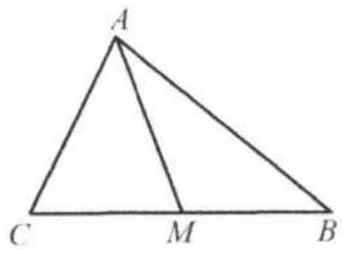
\includegraphics[width=\textwidth]{images/027.jpg}

\section*{Solution}
Extend \(A M\) to \(E\) such that \(A M=M E\).\\
Connect \(C E\).\\
Since \(A M=M E, C M=B M, \angle A M B=\angle E M C\), we have \(\triangle A M B \cong \triangle E M C\).

So \(C E=A B, \angle B A M=\angle C E A\).\\
In triangle \(A C E, C E=A B>A C \quad \angle C A E>\) \(\angle C E A\).

Since \(\angle B A M=\angle C E A, \quad \angle C A M>\angle B A M\).

\end{document}
